\documentclass[11pt]{scrartcl}
\usepackage{graphicx} % Required for inserting images
\usepackage[sexy]{evan}
\usepackage{graphics}
\usepackage{ amssymb }
\usepackage[dvipsnames]{xcolor}
\usepackage{lmodern}


\begin{document}
\title{Problemas Nacionales 2000-2023}
\author{Emmanuel Buenrostro}

\maketitle

\section{Álgebra}

\subsection{P1-P4}
\begin{problem} [2009/4]

    Sea $n > 1$ un entero impar y sean $a_1,a_2,\dots, a_n$ números reales distintos. Sea $M$ el mayor de estos números y sea $m$ el menor de ellos. Muestra que es posible escoger los signos en la expresión $s=\pm a_1\pm a_2\pm \dots \pm a_n$ de manera que \[m< s < M.\]
    
\end{problem}
\begin{problem}
[2010/1] Encuentra todas las ternas de numeros naturales $(a,b,c)$ que cumplan la ecuación $abc=a+b+c+1$
\end{problem}

\begin{problem}
[2012/4] A cada entero positivo se le aplica el siguiente proceso: al número se le resta la suma de sus digitos, y el resultado se divide entre 9. Por ejemplo, el resultado del proceso aplicado a 938 es 102, ya que $(938-(9+3+8)/9=102)$. Aplicado dos veces el proceso a 938 se llega a 11, aplicando tres veces se llega a 1, y aplicado cuatro veces se llega al 0. Cuando a un entero positivo $n$ se le aplica el proceso una o varias veces, se termina en 0. Al número al que se llega antes de llegar al cero, lo llamamos la casa de $n$. ¿Cuántos numeros menores que 26000 tienen la misma casa que el 2012?
\end{problem}

\begin{problem}
[2013/1] Se escriben los números primos en orden $p_1=2, p_2=3, p_3=5,\ldots$ Encuentra todas las parejas de números enteros positivos $a$ y $b$ con $a-b\geq 2$, tales que $p_a-p_b$ divide al numero entero $2(a-b)$.
\end{problem}

\begin{problem}
[2017/4] Un subconjunto $B$ de $\{ 1,2,\ldots ,2017\}$, tiene la propiedad $T$ si 
\begin{center}
\textit{Cada tres números de $B$ son las longitudes de los lados de un triángulo (de área positiva).}
\end{center}
Determina la mayor cantidad de números que puede tener un conjunto $B$ que tenga la propiedad $T$.
\end{problem}

\begin{problem}
[2018/4] Sea $n\geq 2$ un número entero. Para cualquier sucesión $a_1,a_2,\ldots,a_k$ de enteros positivos tales que $a_1+a_2+\ldots+a_k=n$, considera las sumas $S_i=1+2+\ldots+a_i$, para $1\leq i \leq k$. Determina, en términos de $n$, el máximo valor posible del producto $S_1S_2\cdots S_k$
\end{problem}

\begin{problem}
[2021/1] Los números positivos y distintos $a_1,a_2,a_3$ son tres términos consecutivos de una progresión aritmética, y de la misma manera, los números positivos y distintos $b_1,b_2,b_3$ son tres términos consecutivos de una progresión aritemética. ¿Es posible usar tres segmentos con longitudes $a_1,a_2,a_3$ como bases y otros tres segmentos con longitudes $b_1,b_2,b_3$ como alturas (en algún orden), para construir tres rectángulos con la misma área?.
\end{problem}
\begin{problem}
    [2022/1] 
    Un número $x$ es Tlahiuca si existen primos positivos distintos $p_1,p_2,\dots,p_k$ tales que 
\[x=\frac{1}{p_1}+\frac{1}{p_2}+\cdots+\frac{1}{p_k}.\]
Deterimina el mayor número Tlahuica $x$ que satisface las dos siguientes propiedades:
 \begin{itemize} 
 \item  $0< x < 1$. 
 \item  Existe un número entero $0< m\leq 2022$ tal que $mx$ es un número entero. 
 \end{itemize} 
\end{problem}

\begin{problem} [2023/1]
    Encuentre todos los números enteros positivos de cuatro dígitos tales que la suma de los cuadrados de sus dígitos sea el doble que la suma de sus dígitos.
\end{problem}
\subsection{P2-P5}
\begin{problem} [2008/5]

    En los vértices de un cubo están escritos $8$ enteros positivos distintos y en cada una de
las aristas del cubo está escrito el máximo común divisor de los números que están en los
$2$ vértices que forman a la arista. Sean $A$ la suma de los números escritos en las aristas y
$V$ la suma de los números escritos en los vértices. Muestra que $\frac 23 A \leq V$. ¿Es posible que $A = V$ ?
    
\end{problem}
\begin{problem}
[2013/5] Una pareja de enteros es \textit{especial} si es de la forma $(n,n-1)$ o $(n-1,n)$,con $n$ un entero positivo.Sean $n,m$ enteros positivos tales que $(n,m)$ no es una pareja especial. Muestra que $(n,m)$ puede expresarse como suma de dos o mas parejas especiales diferentes si y solo si $$m+n \geq (n-m)^2$$.
\end{problem}

\begin{problem}
[2014/5] Sean $a,b,c$ reales positivos con $a+b+c=3$. Muestra que 
$$\frac{a^2}{a+\sqrt[3]{bc}}+\frac{b^2}{b+\sqrt[3]{ca}}+\frac{c^2}{c+\sqrt[3]{ab}}\geq \frac 3 2$$
\end{problem}

\subsection{P3-P6}
\begin{problem} [2007/3]

    Sean $a,b,c$ números reales positivos tales que $a+b+c=1$. Muestra que 
\[\sqrt{a+bc}+\sqrt{b+ca}+\sqrt{c+ab}\leq 2.\]
    
\end{problem}

\begin{problem} [2009/3]

    Sean $a,b,c$ números reales positivos tales que $abc=1$. Muestra que

\[\frac{a^3}{a^3+2}+\frac{b^3}{b^3+2}+\frac{c^3}{c^3+2}\ge1\text{ y que }\frac1{a^3+2}+\frac1{b^3+2}+\frac1{c^3+2}\le1.\]
    
\end{problem}
\begin{problem}
[2011/3] Sea $n\geq 3$ un entero positivo.Encuentra todas las soluciones $(a_1,a_2,\ldots,a_n)$ de números reales que satisfacen el siguiente sistema de $n$ ecuaciones:
$$a_1^2+a_1-1=a_2$$
$$a_2^2+a_2-1=a_3$$
$$\vdots$$
$$a_{n-1}^2+a_{n-1}-1=a_n$$
$$a_n^2+a_n-1=a_1.$$
\end{problem}

\begin{problem}
[2015/3] Sea $\mathbb{N}=\{ 1,2,3,\ldots \}$ el conjunto de los números enteros positivos. Sea $f: \mathbb{N} \rightarrow \mathbb{N}$ una función, la cual asigna a cada número entero positivo, un número entero positivo. Supón que $f$ satisface las siguientes dos condiciones: 
\begin{itemize}
\item $f(1)=1$
\item Para todos $a,b$ enteros positivos, se cumple que 
$$f(a+b+ab)=a+b+f(ab)$$
Encuentra el valor de $f(2015)$.
\end{itemize}
\end{problem}

\begin{problem}
[2016/3] Encuentra el menor número real $x$ que cumpla todas las siguientes desigualdades: 
$$\lfloor x \rfloor < \lfloor x^2 \rfloor <\lfloor x^3 \rfloor < \ldots < \lfloor x^n \rfloor < \lfloor x^{n+1} \rfloor <\ldots$$
\end{problem}

\begin{problem}
[2020/6] 
    Sea $n\ge 2$ un número entero positivo. Sean $x_1, x_2, \dots, x_n$ números reales no nulos que satisfacen la ecuación
\[\left(x_1+\frac{1}{x_2}\right)\left(x_2+\frac{1}{x_3}\right)\dots\left(x_n+\frac{1}{x_1}\right)=\left(x_1^2+\frac{1}{x_2^2}\right)\left(x_2^2+\frac{1}{x_3^2}\right)\dots\left(x_n^2+\frac{1}{x_1^2}\right). \]
Encuentra todos los valores posibles de $x_1, x_2, \dots, x_n$.
\end{problem}


\section{Geometria}
\subsection{P1-P4}
\begin{problem} [2000/1]

    Existen circunferencias $A,B,C,D$ en el plano tales que las circunferencias $A$ y $B$ son tangentes externamente en $P, B$ y $C$ en $Q, C$ y $D$ en $R$, y $D$ y $A$ en $S$. Las circunferencias $A$ y $C$ no se encuentran, ni tampoco $B$ y $D$.
Muestra que los puntos $P,Q,R,S$ se encuentran en una misma circunferencia.

Supongamos que $A$ y $C$ tienen radio $2, B$ y $D$ tienen radio $3$, y la distancia entre los centros de $A$ y $C$ es $6$. Calcula el área del cuadrilátero $PQRS$.

   
\end{problem}
\begin{problem}[2003/4] 
    Sea $ABCD$ un trapecio con $AB$ paralelo a $DC$. Se toman puntos $P$ y $Q$ en los lados $AB$ y $CD$, respectivamente, tales que $\frac{AP}{PB}=\frac{DQ}{QC}$. Sea $M$ la intersección de $AQ$ con $DP$ y sea $N$ la intersección de $PC$ con $QB$. Muestra que la longitud de $MN$ depende únicamente de las longitudes de $AB$ y $CD$, y calcula su valor.
   \end{problem}
\begin{problem} [2005/1] 
    Sea $O$ el centro de la circunferencia circunscrita al triángulo $ABC$, y sea $P$ un punto cualquiera del segmento $BC$ ($P\neq B$ y $P\neq C$). Supón que la circunferencia circunscrita al triángulo $BPO$ corta al segmento $AB$ en $R$ ($R\neq A$ y $R\neq B$) y que la circunferencia circunscrita al triángulo $COP$ corta al segmento $CA$ en el punto $Q$ ($Q\neq C$ y $Q\neq A$). Muestra que el triángulo $PQR$ que es semejante al triángulo $ABC$ y su ortocentro es $O$. A demás, muestra que las circunferencias circunscritas a los triángulos $BPO$, $COP$, $PQR$ son todas del mismo tamaño.
    \end{problem}
\begin{problem}
[2009/1] Sean $ABC$ un triangulo y $AD$ la altrua sobre el lado $BC$. Tomando a $D$ como centro y a $AD$ como radio,se traza una circunferencia que corta a la recta $AB$ en $P$, y corta a la recta $AC$ en $Q$. Muestra que el triangulo $AQP$ es semejante al triangulo $ABC$.
\end{problem}

\begin{problem}
[2012/1] Sea $C_1$ una circunferencia con centro $O, P$ un punto sobre ella y $l$ la recta tangente a $C_1$ en $P$. Considera un punto $Q$ sobre $l$, distinto de $P$, y sea $C_2$ la circunferencia que pasa por $O, P$ y $Q$. El segmento $OQ$ intersecta a $C_1$ en $S$ y la recta $PS$ intersecta a $C_2$ en un punto $R$ distinto de $P$. Si $r_1$ y $r_2$ son las longitudes de los radios $C_1$ y $C_2$, respectivamente, muestra que 
$$\frac{PS}{SR}=\frac{r_1}{r_2}$$
\end{problem}

\begin{problem}
[2014/4] Sea $ABCD$ un rectangulo con diagonales $AC$ y $BD$. Sean $E$ el punto de interseccion de la bisectriz del angulo $\angle{CAD}$ con el segmento $CD, F$ el punto sobre el segmento $CD$ tal que $E$ es punto medio de $DF$ y $G$ el punto sobre la recta $BC$ tal que $BG=AC$ (con $C$ entre $B$ y $G$). Muestra que la circunferencia que pasa por $D,F$ y $G$ es tangente a $BG$.
\end{problem}

\begin{problem}
[2015/1] Sea $ABC$ un triangulo y sea $H$ su ortocentro. Sea $PQ$ un segmento que pasa por $H$ con $P$ en $AB$, $Q$ en $AC$ y tal que $\angle{PHB}=\angle{CHQ}$. Finalmente en el circuncirculo del triangulo $ABC$, considera $M$ el punto medio del arco $BC$ que no contiene a $A$. Muestra que $MP=MQ$.
\end{problem}

\begin{problem}
[2016/1] Sean $C_1$ y $C_2$ dos circunferencias tangentes externamente en $S$ tales que el radio de $C_2$ es el triple del radio de $C_1$. Sea $l$ una recta que es tangente a $C_1$ en $P$ y tangente a $C_2$ en $Q$, con $P$ y $Q$ distintos de $S$. Sea $T$ el punto de $C_2$ tal que $TQ$ es diametro de $C_2$ y sea $R$ la interseccion de la bisectriz de $\angle{SQT}$ con el segmento $ST$. Demuestra que $QR=RT$.
\end{problem}

\begin{problem}
[2018/1] Sean $A$ y $B$ dos puntos de una recta $l$, $M$ el punto medio del segmento $AB$ y $X$ un punto del segmento $AB$, diferente de $M$. Sea $\Omega$ una semicircunferencia de diametro $AB$. Considera un punto $P$ sobre $\Omega$ y considera $\Gamma$ la circunferencia tangente a $AB$ que pasa por $P$ y por $X$. Sea $Q$ la otra interseccion de $\Gamma$ con $\Omega$. La bisectriz del angulo $\angle{PXQ}$ intersecta a $\Gamma$ en un punto $R$. Sea $Y$ un punto en $l$, tal que $RY$ es perpendicular a $l$. Muestra que $MX>XY$.
\end{problem}
\begin{problem}
[2021/4] Sea $ABC$ un triangulo acutangulo escaleno con $\angle{BAC}=60$ y ortocentro $H$. Sean $\omega_b$ la circunferencia que pasa por $H$ y es tangente a $AB$ en $B$,  y $\omega_c$ la circunferencia que pasa por $H$ y es tangente a $AC$ en $C$. 
\begin{itemize}
\item Prueba que $\omega_b$ y $\omega_c$ solamente tienen a $H$ como punto comun.
\item Prueba que la recta que pasa por $H$ y el circuncentro $O$ del triangulo $ABC$, es una tangente comun a $\omega_b$ y $\omega_c$.
\end{itemize}
\end{problem}

\subsection{P2-P5}
\begin{problem} [2001/5] 
    Sea $ABC$ un triángulo tal que $AB< AC$ y el ángulo $\angle BAC$ es el doble del ángulo $\angle BCA$. EN el lado $AC$ se toma un punto $D$ tal que $CD=AB$. Por el punto $B$ se traza una recta $\ell$ paralela a $AC$. La bisectriz exterior del ángulo en $A$ intersecta a $\ell$ en el punto $M$, y la paralela a $AB$ por el punto $C$ intersecta a $\ell$ en el punto $N$. Muestra que $MD=ND$.
    \end{problem}
\begin{problem} [2002/2]
    Sea $ABCD$ un paralelogramo y $\Gamma$ el circuncírculo del triángulo $ABD$. Sean $E$ y $F$ las intersecciones de $\Gamma$ con los lados $BC$ y $CD$ (o sus prolongaciones), respectivamente. Muestra que el circuncentro del triángulo $CEF$ está en $\Gamma$.
  \end{problem}
\begin{problem} [2003/2] 
    Sean $A$, $B$ y $C$ tres puntos colineales con $B$ entre $A$ y $C$. Sea $\mathcal{Y}$ una circunferencia tangente a $AC$ en $B$, sean $\mathcal{X}$ y $\mathcal{Z}$ las circunferencias de diámetros $AB$ y $BC$, respectivamente. Sea $P$ el punto (además de $B$) en el que se cortan las circunferencias $\mathcal{X}$ y $\mathcal{Y}$; sea $Q$ el otro punto (además de $B$) en el que se cortan las circunferencias $\mathcal{Y}$ y $\mathcal{Z}$. Supón que la recta $PQ$ corta a $\mathcal{X}$ en un punto $R$ distinto de $P$ y que esta misma recta $PQ$ corta a $\mathcal{Z}$ en un punto $S$ distinto de $Q$. Muestra que concurren $AR,$ $CS$ y la tangente común a $\mathcal{X}$ y $\mathcal{Z}$ por $B$.
    \end{problem}
\begin{problem} [2004/5] 
    Sean $\mathcal{A}$ y $\mathcal{B}$ dos circunferencias tales que el centro $O$ de $\mathcal{B}$ esté en $\mathcal{A}$. Sean $C$ y $D$ los dos puntos de intersección de las circunferencias. Se toman un punto $A$ en $\mathcal{A}$ y un punto $B$ en $\mathcal{B}$ tales que $AC$ es tangente a $\mathcal{B}$ en $C$ y $BC$ es tangente a $\mathcal{A}$ en el mismo punto $C$. El segmento $AB$ corta de nuevo a $\mathcal{B}$ en $E$ y ese mismo segmento corta de nuevo a $\mathcal{A}$ en $F$. La recta $CE$ vuelve a cortar a $\mathcal{A}$ en $G$ y la recta $CF$ corta a la recta $GD$ en $H$. Muestra que el punto de intersección de $GO$ y $EH$ es el centro de la circunferencia circunscrita al triángulo $DEF$.
   \end{problem}
\begin{problem} [2006/2] 
    Sea $ABC$ un triángulo rectángulo con ángulo recto en $A$, tal que $AB\lt AC$. Sean $M$ el punto medio de $BC$ y $D$ la intersección de $AC$ con la perpendicular a $BC$ que pasa por $M$. Sea $E$ la intersección de la paralela a $AC$ que pasa por $M$ con la perpendicular a $BD$ que pasa por $B$. Muestra que los triángulos $AEM$ y $MCA$ son semejantes si y solo si $\angle ABC=60^o$.
    \end{problem}
\begin{problem} [2006/5] 
    Sean $ABC$ un triángulo acutángulo y $AD$, $BE$ y $CF$ sus alturas. La circunferencia con diámetro $AD$ corta a los lados $AB$ y $AC$ en $M$ y $N$, respectivamente. Sean $P$ u $Q$ los puntos de intersección de $AD$ con $EF$ y $MN$, respectivamente. Muestra que $Q$ es el punto medio de $PD$.
    \end{problem}
\begin{problem} [2007/2] 
    Dado un triángulo equilátero $ABC$, encuentra todos los puntos $P$ del plano que cumplan $\angle APB=\angle BPC$.
    \end{problem}

 \begin{problem} [2008/2] 
    Considera una circunferencia $\Gamma$, un punto $A$ fuera de $\Gamma$ y las tangentes $AB$, $AC$ a $\Gamma$ desde
$A$, con $B$ y $C$ los puntos de tangencia. Sea $P$ un punto sobre el segmento $AB$, distinto de
$A$ y de $B$. Considera el punto $Q$ sobre el segmento $AC$ tal que $P Q$ es tangente a $\Gamma$, y a los
puntos $R$ y $S$ que están sobre las rectas $AB$ y $AC$, respectivamente, de manera que $RS$
es paralela a $P Q$ y tangente a $\Gamma$. Muestra que el producto de las áreas de los triángulos
$APQ$ y $ARS$ no depende de la elección del punto $P$ .
    \end{problem}
 
\begin{problem}
[2009/5] Considera un triangulo $ABC$ y un punto $M$ sobre el lado $BC$. Sea $P$ la interseccion de las perpendiculares a $AB$ por $M$ y a $BC$ por $B$, y sea $Q$ la interseccion de las perpendiculares a $AC$ por $M$ y a $BC$ por $C$. Muestra que $PQ$ es perpendicular a $AM$ si y solo si $M$ es punto medio de $BC$. 
\end{problem}

\begin{problem}
[2010/5]Sea $ABC$ un triángulo acutángulo con $AB \neq AC$, $M$ el punto medio de $BC$ y $H$ el otrocentro de $ABC$. La circunferencia que pasa por $B$, $H$ y $C$ corta a la mediana de $AM$ en $N$. Muestra que $\angle ANH = 90^{\circ}$.
\end{problem}

\begin{problem}
[2011/2] Sea $ABC$ un triángulo acutángulo con sus vértices sobre la circunferencia $\zeta$. Sea $l$ la recta tangente a $\zeta$ en el punto $A$. La circunferencia con centro en $B$ y radio $BA$ interseca a la recta $l$ en $D$ y a la recta $AC$ en $E$. Muestra que la recta $DE$ pasa por el ortocentro del triángulo $ABC$.
\end{problem}

\begin{problem}
[2013/2]Sea $ABCD$ un parelelogramo con un ángulo obtuso en $A$. Sea $P$ un punto sobre el segmento $BD$ de manera que la circunferencia con centro en $P$ y que pasa por $A$, corte a la recta $AD$ en $A$ y $Y$, y corte a la recta $AB$ en $A$ y $X$. La recta $AP$ intersecta a $BC$ en $Q$ y a $CD$ en $R$, respectivamente. Muestra que $\angle XPY = \angle XQY + \angle XRY$.
\end{problem}

\begin{problem}
[2015/5]Sea $I$ el incentro de un triángulo acutángulo $ABC$. La recta $AI$ corta por segunda vez al circuncírculo del triángulo $BIC$ en $E$. Sean $D$ el pie de la altura desde $A$ sobre $BC$ y $J$ la reflexión de $I$ con respecto a $BC$. Muestra que los puntos $D$, $J$ y $E$ son colineales.
\end{problem}

\begin{problem}
[2017/5]Sobre una circunferencia $\Gamma$ se encuentran los puntos $A$, $B$, $N$, $C$, $D$ y $M$ colocados en el sentido de las manecillas del reloj de manera que $M$ y $N$ son los puntos medios de los arcos $DA$ y $BC$ (recorridos en el sentido de las manecillas del reloj). Sea $P$ la intersección de los segmentos $AC$ y$BD$; y sea $Q$ un punto sobre $MB$ de manera que las rectas $PQ$ y $MN$ son perpendiculares. Sobre el segmento $MC$ se considera un punto $R$ de manera que $QB = RC$. Muestra que $AC$ pasa por el punto medio del segmento $QR$.
\end{problem}

\begin{problem}
[2019/2]Sea $H$ el ortocentro del triángulo acutángulo $ABC$ y $M$ el punto medio de $AH$. La recta $BH$ corta a $AC$ en $D$. Considera un punto $E$ de manera que $BC$ sea mediatriz del segmento $DE$. Los segmentos $CM$ y $AE$ se cortan en $F$. Muestra que $BF$ es perpendicular a $CM$.
\end{problem}

\begin{problem}
[2020/2] Sea $ABC$ un triángulo con incentro $I$. La recta $BI$ corta a $AC$ en $D$. Sean $P$ un punto en $CI$ tal que $DI = DP$ ($P \neq I$), $E$ la segunda intersección del segmento $BC$ con el circuncírculo del triángulo $ABD$ y $Q$ la segunda intersección de la recta $EP$ con el circuncírculo del triángulo $AEC$. Muestra que $\angle PDQ = 90^{\circ}$.
\end{problem}

\begin{problem}
[2021/2] Sea $ABC$ un triángulo tal que $\angle ACB > 90^{\circ}$ y sea $D$ el punto de la recta $BC$ tal que $AD$ es perpendicular a $BC$. Considera $\Gamma$ la circunferencia de diámetro $BC$. Una recta que pasa por $D$ es tangente a la circunferencia $\Gamma$ en $P$, corta al lado $AC$ en $M$ (quedando $M$ entre $A$ y $C$) y corta al lado $AB$ en $N$.
Demuestra que $M$ es el punto medio de $DP$ si, y solo si $N$ es punto medio de $AB$.
\end{problem}
\begin{problem} [2023/5]
    Sea $ABC$ un triangulo acutangulo, $\Gamma$ su circuncirculo y $O$ su circuncentro. Sea $F$ el punto en $AC$ tal que $\angle COF=\angle ACB$, donde $F$ y $B$ estan de lados opuestos respecto a $CO$. La recta $FO$ corta a $BC$ en $G$. La paralela a $BC$ por $A$ intersecta a $\Gamma$ de nuevo en $M$. Las rectas $MG$ y $CO$ se cortan en $K$. Demuestra que los circuncirculos de los triangulos $BGK$ y $AOK$ concurren en $AB$.
\end{problem}
\subsection{P3-P6}
\begin{problem} [2000/6]
    Sea $ABC$ un triángulo con $\angle B > 90^o$ tal que existe un punto $H$ en el lado $AC$ con $AH = BH$ y BH perpendicular a $BC$. Sean $D$ y $E$ los puntos medios de $AB$ y $BC$ respectivamente. La recta que pasa por $H$ paralela a $AB$ corta a $DE$ en $F$. Muestra que $\angle BCF = \angle ACD$. 
\end{problem}
\begin{problem}[2001/3]
    En un cuadrilátero $ABCD$ inscrito en una circunferencia llamemos $P$ al punto de intersección de las diagonales $AC$ y $BD$, y sea $M$ el punto medio de $CD$. Una circunferencia que pasa por $P$ y que es tangente a $CD$ en $M$ corta a $BD$ y a $AC$ en los puntos $Q$ y $R$, respectivamente. Se toma un punto $S$ en el segmento $BD$ de tal manera que $BS=DQ$. Por $S$ se traza una paralela a $AB$ que corta a $AC$ en un punto $T$. Muestra que $AT=RC$.
    
    
\end{problem}
\begin{problem}[2002/6]
    Sea $ABCD$ un cuadrilátero con $AD$ paralelo a $BC$, los ángulos en $A$ y $B$ rectos y con el ángulo $\angle CMD$ recto, donde $M$ es el punto medio de $AB$. Sean $K$ el pie de la perpendicular a $CD$ que pasa por $M$, $P$ el punto medio de intersección de $AK$ con $BD$ y $Q$ el punto de intersección de $BK$ con $AC$. Muestra que el ángulo $\angle AKB$ es recto y que $\frac{KP}{PA} + \frac{KQ}{QB}=1$.    
\end{problem}
\begin{problem} [2004/1]
    
    Sean $Z$ y $Y$ los puntos de tangencia del incírculo del triángulo $ABC$ con los lados $AB$ y $CA$, respectivamente. La paralela a $YZ$ por el punto medio $M$ del lado $BC$ corta a $CA$ en $N$. Sea $L$ el punto del segmento $CA$ tal que $NL=AB$ (con $L$ y $A$ del mismo lado con respecto a $N$). La recta $ML$ corta a $AB$ en $K$. Muestra que $KA=NC$.
\end{problem}
\begin{problem} [2005/6]
    Sea $ABC$ un triángulo y $AD$ la bisectriz del ángulo $\angle BAC$, con $D$ un punto del lado $BC$. Sea $E$ un punto del segmento $BC$ tal que $BD=EC$. Por $E$ se traza $\ell$, la recta paralela a $AD$. Sea $P$ un punto en $\ell$ y dentro del triángulo $ABC$. Sea $G$ el punto donde la recta $BP$ corta al lado $AC$ y sea $F$ el punto donde la recta $CP$ corta al lado $AB$. Muestra que $BF=CG$.
\end{problem}
\begin{problem} [2007/6]
    Sea $ABC$ un triángulo tal que $AB > AC > BC$. Sea $D$ un punto sobre el lado $AB$ de tal
manera que $CD = BC$, y sea $M$ el punto medio del lado $AC$. Muestra que $BD = AC$ si
y sólo si $\angle BAC = 2\angle ABM$ .
\end{problem}
\begin{problem}[2008/6]
    Las bisectrices internas de los ángulos $A, B$ y $C$ de un triángulo $ABC$ concurren en $I$
y cortan al circuncírculo de $ABC$ en $L, M, N$, respectivamente. La circunferencia de
diámetro $IL$ corta al lado $BC$, en $D$ y $E$; la circunferencia de diámetro $IM$ corta al lado
$CA$ en $F$ y $G$; la circunferencia de diámetro $IN$ corta al lado $AB$ en $H$ y $J$. Muestra que
$D, E, F , G, H, J$ están sobre una misma circunferencia.
    
\end{problem}
\begin{problem}
[2010/3] Sean $C_1$ y $C_2$ dos circunferencias tangentes exteriormente en un punto $A$. Se traza una recta tangente a $C_1$ en $B$ y secante a $C_2$ en $C$ y $D$; luego se prolonga el segmneto $AB$ hasta intersectar a $C_2$ en un punto $E$. Sea $F$ el punto medio de arco $CD$ sobre $C_2$ que no contiene a $E$ y sea $H$ la interseccion de $BF$ con $C_2$. Muestra que $CD,AF$ y $AH$ son concurrentes.
\end{problem}

\begin{problem}
[2011/6] Sean $C_1$ y $C_2$ dos circunferencias de radios diferentes que se cortan en los puntos $A$ y $B$. Consideramos un punto $C$ sobre la recta $AB$ de modo que $B$ queda entre $A$ y $C$. Sean $P$ y $Q$ sobre $C_1$ y $C_2$, respectivamente, tales que $CP$ es tangente a $C_1$ y $CQ$ tangente a $C_2$. $P$ no esta adentro de $C_2$ y $Q$ no esta dentro de $C_1$. La recta $PQ$ corta de nuevo a $C_1$ en $R$ y a $C_2$ en $S$, ambos puntos distintos de $B$. Supongamos que $CR$ corta de nuevo a $C_1$ en $X$ y $CS$ corta de nuevo a $C_2$ en $Y$. Sea $Z$ un punto sobre la recta $XY$. Muestra que $SZ$ es paralela a $QX$ si y solo si $PZ$ es paralela a $RX$.
\end{problem}

\begin{problem}
[2012/6] Considera un triangulo acutangulo $ABC$ con circuncirculo $\Gamma$. Sean $H$ el ortocentro del triangulo $ABC$ y $M$ el punto medio de $BC$. Las rectas $AH,BH$ y $CH$ cortan por segunda vez a $\Gamma$ en $D,E$ y $F$, respectivamente; la recta $MH$ corta a $\Gamma$ en $J$ de manera que $H$ queda entre $M$ y $J$. Sean $K$ y $L$ los incentros de los triangulos $DEJ$ y $DFJ$, respectivamente. Muestra que $KL$ es paralela a $BC$. 
\end{problem}

\begin{problem}
[2013/6] Sea $A_1A_2\ldots A_8$ un octagono convexo, es decir, un octagono donde todos sus angulos internos son menores que 180. Además los lados del octagono tienen la misma longitud y cada par de lados opuestos son paralelos. Para cada $i=1,2,\ldots,8$ definamos el punto $B_i$ como la interseccion  del segmento $A_iA_{i+4}$ con el segmento $A_{i-1}A_{i+1}$ donde $A_{j+8}=A_j$ y $B_{j+8}=B_j$ para todo numero entero $j$ Muestra que para algun numero $i$ de entre los numeros 1,2,3 y 4 se cumple que 
$$\frac{|A_iA_{i+4}|}{B_iB_{i+4}}\geq \frac 3 2$$
\end{problem}

\begin{problem}
[2014/3] Sean $\Gamma_1$ una circunferencia y $P$ un punto fuera de $\Gamma_1$.Las tangentes desde $P$ a $\Gamma_1$ tocan a la circunferencia en los puntos $A$ y $B$. Considera $M$ el punto medio del segmento $PA$ y $\Gamma_2$ la circunferencia que pasa por los puntos $P,A$  y $B$. La recta $BM$ intersecta de nuevo a $\Gamma_2$ en el punto $C$, la recta $CA$ interesecta de nuevo a $\Gamma_1$ en el punto $D$, el segmento $DB$ intersecta de nuevo a $\Gamma_2$ en el punto $E$y la recta $PE$ intersecta a $\Gamma_1$ en el punto $F$ (con $E$ entre $P$ y $F$). \\
Muestra que las rectas $AF,BP$ y $CE$ concurren.
\end{problem}

\begin{problem}
[2016/6] Sea $ABCD$ un cuadrilatero inscrito en una circunferencia, $l_1$ la recta paralela a $BC$ que pasa por $A$ y $l_2$ la recta paralela a $AD$ que pasa por $B$. La recta $DC$ corta a $l_1$ y $l_2$ en los puntos $E$ y $F$, respectivamente. La recta perpendicular a $l_1$ que pasa por $A$ corta a $BC$ en $P$ y la recta perpendicular a $l_2$ por $B$ corta a $AD$ en $Q$. Sean $\Gamma_1$ y $\Gamma_2$ las circunferencias que pasan por los vertices de los triangulos $ADE$ y $BFC$, respectivamente. Demuestra que $\Gamma_1$ y $\Gamma_2$ son tangentes si y solo si $DP$ es perpendicular a $CQ$. 
\end{problem}

\begin{problem}
[2017/3] Sea $ABC$ un triangulo acutangulo cuyo ortocentro es el punto $H$. La circunferencia que pasa por los puntos $B,H$ y $C$ vuelve  a intersectar a las rectas $AB$ y $AC$ en los puntos $D$ y $E$, respectivamente. Sean $P$ y $Q$ los puntos de interseccion de $HB$ y $HC$ con el segmento $DE$ , respectivamente. Se consideran los puntos $X$ e $Y$ (distintos de $A$) que estan sobre la recta $AP$ y $AQ$, respectivamente, de manera que los puntos $X,A,H$ y $B$ estan sobre un circulo y los puntos $Y,A,H$ y $C$ estan sobre un circulo. Muestra que las rectas $XY$ y $BC$ son paralelas.
\end{problem}

\begin{problem}
[2018/6] Sea $ABC$ un triangulo acutangulo y $\Omega$ la circunferencia que pasa por los puntos $A,B$ y $C$. La bisectriz del angulo en $B$ corta a $\Omega$ en $M$ y la bisectriz del angulo en $C$ corta a $\Omega$ en $N$. Sea $I$ el punto de interseccion de las bisectrices anteriores. Considera $M'$ y $N'$ las reflexiones de $M$ y $N$ con respecto a $CA$ y $AB$ respectivamente. Muestra que el centro de la circunferencia que pasa por los puntos $I,M'$ y $N'$ esta en la altura del triangulo $ABC$ que pasa por $A$.
\end{problem}

\begin{problem}
[2019/6] Sea $ABC$ un triangulo con $\angle{BAC}=45$ con ortocentro $H$, circuncentro $O$ y circuncirculo $\Gamma$. Sea $P$ un punto de $\Gamma$ tal que el circuncirculo del triangulo $PHB$ es tangente a $BC$ en $B$. Sean $X$ y $Y$ los circuncentros de los triangulos $PHB$ y $PHC$, respectivamente. Sean $O_1$ y $O_2$ los circuncentros de los triangulos $PXO$ y $PYO$, respectivamente. Muestre que $O_1$ y $O_2$ son puntos de las rectas $AB$ y $AC$, respectivamente.
\end{problem}

\begin{problem}
    [2022/6] 
    Encuentra todos los enteros $n\geq 3$ tales que existe un polígono convexto de $n$ lados $A_1A_2\dots A_n$ que tenga las siguientes características:
 \begin{itemize} 
 \item  Todos los ángulos internos de $A_1A_2\dots A_n$ son iguales. 
 \item  No todos los lados de $A_1A_2\dots A_n$ son iguales.
 \item  Existe un triángulo $T$ y un punto $O$ en el interior de $A_1A_2\dots A_n$ tal que los $n$ triángulos $OA_1A_2, OA_2A_3,\dots OA_nA_1$ son todos semejantes a $T$.
 \end{itemize} 
\end{problem}
\begin{problem} [2023/3]
    Sea $ABCD$ un cuadrilatero convexo. Si $M,N,K$ son los puntos medios de los segmentos $AB,BC$ y $CD$ respectivamente, y ademas existe un punto $P$ dentro del cuadrilatero $ABCD$ tal que $\angle BPN =\angle PAD$ y $\angle CPN=\angle PDA$ demuestre que $AB\cdot CD =4PM \cdot PK$
\end{problem}
\section{Numeros}

\subsection{P1-4}
\begin{problem}[2000/4]
    Sean $a$ y $b$ enteros positivos que no son múltiplos de $5$. Se construye una sucesión de enteros como sigue: el primer término es $5$, y cada término siguiente se obtiene multiplicando el anterior por $a$ y añadiendo $b$. (Por ejemplo, si $a = 2$ y $b = 4$, los tres primeros términos son $5,14,32$.) ¿Cuál es el máximo número posible de números primos en la secuencia que pueden aparecer antes de que haya un término compuesto? 
\end{problem}
\begin{problem} [2001/1]
    Encuentra todos los números enteros de $7$ dígitos que son múltiplos de $3$ y de $7$, y cada uno de cuyos dígitos es $3$ o $7$.
\end{problem}
\begin{problem} [2001/4]
    Dados dos enteros positivos $n$ y $a$ se forma una lista de $2001$ números enteros como sigue: El primer número es $a$; a partir del segundo, cada número es el residuo que se obtiene al dividir el cuadrado del anterior entre $n$. A los números de la lista se les ponen los signos $+$ y $-$ alternadamente empezando con $+$. Los números con signo así obtenidos se suman y a esa suma se le llama suma final para $n$ y $a$. ¿Para qué números enteros $n\geq 5$ existe alguna $a$ tal que $2\leq a \leq \frac{n}{2}$ y la suma final para $n$ y $a$ es positiva?
\end{problem}
\begin{problem}[2003/1]
    Dado un número entero $k$ de dos o más cifras, se forma otro número entero $m$ insertando un cero entre la cifra de las unidades y la de las decenas de $k$. Encuentra todos los números $k$ para los cuales $m$ resulta ser un múltiplo de $k$.
\end{problem}
\begin{problem} [2004/1]
    
    Encuentra todos los números primos $p$, $q$, $r$ con $p< q< r$, tales que $25pq+r=2004$ y que $pqr+1$ sea un cuadrado perfecto.
\end{problem}
\begin{problem}
    [2006/1]
    Sea $ab$ un número entero de dos digitos. Un entero positivo $n$ es "pariente" de $ab$ si el digito de las unidades de $n$ tambien es $b$, y los otros digitos de $n$ son distintos de cero y suman $a$. Por ejemplo los parientes de 31 son 31,121,211, 1111. Encuentra todos los números de dos digitos que dividen a todos sus parientes.
\end{problem}
\begin{problem}
    [2007/1]
    Encuentra todos los enteros positivos $N$ con la siguiente propiedad: entre todos los divisores positivos de $N$ hay $10$ números consecutivos pero no $11$.
\end{problem}
\begin{problem}
    [2007/4]
    Para un entero positivo $n$ se definen: $n_1$ como la suma de los dígitos de $n$, $n_2$ como la suma de los dígitos de $n_1$ y $n_3$ como la suma de los dígitos de $n_2$. Por ejemplo para $n=199,n_1=19,n_2=199_2=10$ y $n_3=199_3=1$. Encuentra todas las parejas de enteros positivos $(m,n)$ tales que $m+n=2007$ y $m_3+n_3=2007_3$.
\end{problem}
\begin{problem}
    [2008/1]
    Sean $1 = d_1 < d_2 < d_3 < \dots < d_k = n$ los divisores del entero positivo n. Encuentra todos
los números $n$ tales que $n = d_2^2+d_3^3$.
\end{problem}
\begin{problem}
[2011/4] Encuentra el menor entero positivo tal que al escribirlo en notacion decimal utiliza exactamente dos digitos distintos y que es divisible entre cada uno de los números del 1 al 9.
\end{problem}

\begin{problem}
[2015/4] Sea $n$ un entero positivo. María escribe las $n^3$ ternas que se pueden formar tomando tres enteros, no necesariamente distintos, entre 1 y $n$, incluyendolos. Despues, para cada una de las ternas, Maria determina el mayor (o los mayores, en caso de que haya mas de uno) y borra los demas. Por ejemplo, en la terna $(1,3,4)$ borrara los números $1$ y $3$, mientras que en la terna $(1,2,2)$ borrara solo el número 1. \\
Muestra que, al terminal este proceso, la cantidad de numeros que quedan escritos en el pizarron no puede ser igual al cuadrado de un número entero.
\end{problem}

\begin{problem}
[2016/4] Decimos que un numero entero no-negativo $n$ "contiene" a otro numero entero no-negativo $m$, si los digitos de su expansion (o desarrollo) decimal aparecen en forma consecutiva en la expansion (o desarrollo) decimal de $n$. Por ejemplo, 2016 contiene a 2,0,1,6,20,16,201 y 2016. Determina el mayor numero entero $n$ que no contiene a ningun multiplo de 7.
\end{problem}

\begin{problem}
[2019/1] Un número $m \geq 1$ es mexica si es de la forma $n^{d(n)}$, donde $n$ es un entero positivo y $d(n)$ es la cantidad de enteros positivos que dividen a $n$. Encuentra todos los números mexicas menores que 2019.
\end{problem}

\begin{problem}
[2019/4] Una lista de enteros positivos es buena si el elemento maimo de la lista aparece exactamente una vez. Una sublista es una lista formada por varios elementos consecutivos de la lista. Por ejemplo, en la lista 10,34,34,22,30,22, la sublista 22,30,22 es buena, mientras que la sublista 10,34,34,22 no es buena. Una lista es muy buena si todas sus sublistas son buenas. Enceuntra el menor entero positivo $k$ tal que es posible crear una lista muy buena con 2019 elementos, en la cual se usen exactamente $k$ valores distintos.
\end{problem}

\begin{problem}
[2020/1]A un conjunto de 5 enteros positivos, se le llama virtual si el máximo común divisor de cualesquiera 3 de sus elementos es mayor que 1, pero el máximo común divisor de cualesquiera 4 de sus elementos es igual a 1. Demuestra que en cualquier conjunto virtual, el producto de sus 5 elementos tiene al menos 2020 divisores positivos distintos.
\end{problem}

\subsection{P2-5}
\begin{problem}
    [2002/5]
    Tres números enteros distintos forman una terna compatible si alguno de ellos, digamos $n$, cumple que cada uno de los otros dos es, o bien divisor, o bien múltiplo de $n$. Para cada terna compatible de números entre $1$ y $2002$ se calcula la suma de los tres números de la terna. ¿Cuál es la mayor suma obtenida? ¿Cuáles son las ternas en las que se obtiene suma máxima?
\end{problem}
\begin{problem}
    [2004/2]
    ¿Cuál es la mayor cantidad de enteros positivos que se pueden encontrar de manera que cualesquiera dos de ellos $a$ y $b$ (Con $a\neq b$) cumplan que $\left| a-b \right|\geq \frac{ab}{100}$?
\end{problem}
\begin{problem}
    [2005/5]
    Sea $N$ un número entero mayor que $1$. En cierta baraja de $N^3$ cartas, cada carta está pintada de uno de $N$ colores distintos, tiene dibujada una de $N$ posibles figuras,¡ y tiene escrito un número entero del $1$ al $N$ (no hay dos cartas idénticas). Una colección de cartas de la baraja se llama completa si tiene cartas de todos los colores, o si entre sus cartas aparecen todas las figuras o todos los números. ¿Cuántas colecciones no completas tienen la propiedad de que, al añadir cualquier otra carta de la baraja, se vuelven completas?
\end{problem}
\begin{problem}
    [2009/2] 
    En cajas marcadas con los números $0,1,2,\dots$ se van a colocar todos los enteros positivos de acuerdo con las siguientes reglas:

Si $p$ es un número primo, este se coloca en la caja con el número $1$. 

Si el número $a$ se coloca en la caja con el número $m_a$ y $b$ se coloca en la caja con el número $m_b$, entonces el producto de $a$ y $b$, es decir $ab$, se coloca en la caja con el número $am_b+bm_a$.

Encuentra todos los enteros positivos $n$ que cuando se coloquen queden en la caja con el número $n$.
\end{problem}
\begin{problem}
[2014/2]Un entero positivo $a$ se reduce a un entero positivo $b$, si al dividir $a$ entre su dígito de las unidades se obtiene $b$. Por ejemplo, 2015 se reduce a ${2015 \over 5} = 403$. Encuentra todos los enteros positivos que, mediante algunas reducciones, llegan al número 1. Por ejemplo, el número 12 es uno de tales enteros pues 12 se reduce a 6 y se se reduce a 1.
\end{problem}

\begin{problem}
[2016/2]Una pareja de enteros positivos $m, n$ es guerrera si existen enteros positivos $a, b, c, d$ con $m = ab$, $n = cd$ y $a + b = c + d$. Por ejemplo, la pareja 8, 9 es guerrera pues $8 = 4 \times 2$, $9 = 3 \times 3$ y $4 + 2 = 3 + 3$. Se coloren todos los enteros positivos de la siguiente manera:

- Empezamos coloreando el 3 y el 5.

- Después, si algún entero positivo no está coloreado y este tiene una pareja guerrera que ya está coloreada, entonces lo coloreamos.
\end{problem}

\begin{problem}
[2017/2]Un conjunto de $n$ números enteros positivos distintos es equilibrado, si el promedio de cualesquiera $k$ números del conjunto es un número entero, para toda $1 \leq k \leq n$. Encuentra la mayor suma que pueden tener los -elementos de un conjunto equilibrado, con todos sus elementos menores o iguales que 2017.

\end{problem}

\begin{problem}
[2018/5] Sea $n\geq 5$ un número entero y considera un $n$-agono regular. Originalmente , Macho se encuentra en un vertice del $n$-agono, en el cual pondra una bandera. El comenzara a moverse entre los vertices del n-agono, siempre en el sentido de las manecillas del reloj. Primero se movera una posicion y colocara una bandera, luego, se movera dos posiciones y colocara otra bandera, luego, etcetera, hasta que en el ulitmo movimiento se movera $n-1$ posiciones y colocara una bandera, de manera que colocara $n$ banderas en total. ¿Para que valores de $n$, Nacho colocara una bandera en cada uno de los $n$ vertices?.
\end{problem}

\begin{problem}
[2020/5] Una cuarteta de enteros positivos distintos $\{ a,b,c,d\}$, se dice que es pandemica si hay 2 de ellos tales que su producto es multiplo del maximo comun divisor de los otros 2. Por ejemplo, la cuarteta $\{ 4,6,2,8 \}$ es pandemica pues el maximo comun divisor de 2 y 6 es 2, y este divide a $4 \times 8 =32$. \\
Encuentra el maximo valor de $n$, para el cual toda cuarteta de enteros positivos dsitintos menores o iguales que $n$ es pandemica.
\end{problem}

\begin{problem}
[2021/5] Para cada entero $n>0$ con expansion decimal $\overline{a_1a_2\ldots a_k}$ definimos a $s(n)$ como sigue:
\begin{itemize}
\item Si $k$ es par, $s(n)=\overline{a_1a_2}+\overline{a_3a_4}+\ldots+\overline{a_{k-1}a_k}$
\item Si $k$ es impar, $s(n)=a_1+\overline{a_2a_3}+\ldots+\overline{a_{k-1}a_k}$
\end{itemize}
Por ejemplo, si $n=123$ entonces $s(n)=1+23=24$ y si $n=2021$ entonces $s(n)=20+21=41$.\\
Decimos que $n$ es digital si $n$ es mutliplo de $s(n)$. Muestra que entre cualesquiera $198$ enteros positivos consecutivos, todos ellos menores a $2000021$, hay uno de ellos que es digital.
\end{problem}
\begin{problem}
    [2022/5] 
    Sea $n>1$ un entero positivo y sean $d_1< d_2< \dots< d_m$ sus $m$ divisores positivos de manera que $d_1=1$ y $d_m=n$. Lalo escribe los siguientes $2m$ números en un pizarrón:
\[d_1,d_2,\dots,d_m,d_1+d_2,d_2+d_3,\dots,d_{m-1}+d_m,N\]
donde $N$ es un entero positivo. Después Lalo borra los números repetidos (por ejemplo, si un número aparece dos veces, él borrará uno de los dos). Después de esto, Lalo nota que los números en el pizarrón son precisamente la lista completa de divisores positivos de $N$. Encuentra todos los posibles valores del entero positivo $n$.
    
\end{problem}
\subsection{P3-6}
\begin{problem}
    [2000/3]
    Dado un conjunto $A$ de enteros positivos, el conjunto $A'$ se compone de los elementos de $A$ y de todos los enteros positivos que se pueden obtener de la siguiente manera: \\
Se escriben algunos elementos de $A$ uno tras otro sin repetir, se escribe un signo $+ $ o $-$ antes de cada uno de ellos, y se evalúa la expresión obtenida. El resultado se incluye en $A'$. \\
Por ejemplo, si $A = \{2,8,13,20\}$, los números $8$ y $14 = 20-2+8$ son elementos de $A'$. \\
El conjunto $A''$ se construye a partir de $A'$ de la misma manera. \\
Hallar el menor número posible de elementos de $A$, si $A''$ contiene todos los enteros de $1$ a $40$. 
\end{problem}
\begin{problem}
    [2002/3] 
    Sea $n$ un entero positivo. Entre los divisores positivos de $n^2$, ¿Hay más de la forma $4k+1$ o $4k-1$?
\end{problem}
\begin{problem}
    [2003/6]
    Dado un número entero $n$, un cambio sensato consiste en sustituir $n$ por $2n+1$ o $3n+2$. Dos enteros positivos $a$ y $b$ se llaman compatibles si existe un entero que se puede obtener haciendo uno o más cambios sensatos, tanto a partir de $a$, como a partir de $b$. Encuentra todos los enteros positivos compatibles con $2003$ menores que $2003$.
\end{problem}
\begin{problem}
    [2005/3] 
    Determina todas las parejas $(a,b)$ de números enteros distintos de cero para las cuales es posible encontrar un entero entero positivo $x$ primo relativo con $b$ y un entero cualquiera $y$, tales que en la siguiente lista hay una infinidad de números enteros:
\[\frac{a+xy}{b},\frac{a+xy^2}{b^2},\frac{a+xy^3}{b^3},\dots,\frac{a+xy^n}{b^n},\dots\]
\end{problem}
\begin{problem}
    [2006/6] Sea $n$ la suma de los digitos de un entero positivo $A$. Decimos que $A$ es surtido si cada uno de los enteros $1,2,3, \ldots, n$es la suma de algunos digitos de $A$. Muestra que si $1,2,\ldots, 8$ son sumas de algunos digitos de un entero $A$, entonces $A$ es surtido. Si $1,2,\ldots, 7$ son sumas de algunos digitos de $A$, ¿ es $A$ necesariamente surtido?. 
\end{problem}
\begin{problem}
[2010/6] Sean $p,q,r$ numeros primos positivos distintos. Muestra que si $pqr$ divide a $$(pq)^r+(qr)^p+(rp)^q-1$$ 
entonces $(pqr)^3$ divide a 
$$3((pq)^r+(qr)^p+(rp)^q-1)$$
\end{problem}

\begin{problem}
[2012/3]Muestra que entre cualesquiera 14 números enteros positivos consecutivos siempre hay 6 números tales que cualesquiera dos de ellos son primos relativos.
\end{problem}
\begin{problem}
[2013/3]¿Cuál es la mayor cantidad de elementos que puedes tomar del conjunto de números enteros $\{1, 2, ..., 2012, 2013\}$, de tal manera que entre ellos no haya tres distintos, digamos $a, b, c$ tales que $a$ sea divisor o múltiplo de $b-c$.
\end{problem}

\begin{problem}
[2014/6] Para cada entero positivo $n$, sea $d(n)$ la cantidad de divisores positivos de $n$. Por ejemplo, los divisores positivos de 6 son 1,2,3 y 6, por lo que $d(6)=4$. Encuentra todos los enteros positivos $n$ tales que 
$$n+d(n)=d(n)^2$$
\end{problem}

\begin{problem}
[ 2015/6] Sea $n$ un entero positivo y sean $d_1,d_2,\ldots, d_k$ todos sus divisores positivos ordenados de menor a mayor. Considera el número 
$$f(n)=(-1)^{d_1}d_1+(-1)^{d_2}d_2+\cdots+(-1)^{d_k}d_k$$
Por ejemplo los divisores positivos de 10 son 1,2,5 y 10, asi que 
$$f(10)=(-1)^1\cdot 1+(-1)^2 \cdot 2+(-1)^5\cdot 5 +(-1)^10\cdot 10=6$$
Supon que $f(n)$ es una potencia de 2. Muestra que si $m$ es un entero mayor que 1, entonces $m^2$ no divide a $n$.
\end{problem}

\begin{problem}
[2018/3]Una sucesión $a_2, a_3, ..., a_n$ de enteros positivos se dice campechana, si para cada $i$ tal que $2 \leq i \leq n$, se tiene que exactamente $a_i$ elementos de la sucesión son primos relativos con $i$. Decimos que el tamaño de la sucesión es n-1. Sea $m=p_1p_2...p_k$ donde $p_1, p_2, ..., p_k$ son números primos distintos y $k \geq 2$. Demuestra que existen al menos dos sucesiones campechanas de tamaño $m$.
\end{problem}
\begin{problem}
    [2022/3] 
    Sea $n>1$ un entero y sean $d_1< d_2< \dots< d_m$ la lista completa de sus divisores positivos, incluyendo $1$ y $n$. Los $m$ instrumentos de una orquesta matemática se disponen a tocar una pieza musical de $m$ segundos, donde el instrumento $i$ tocará una nota de tono $d_i$ durante $s_i$ segundos (no necesariamente consecutivos), donde $d_i$ y $s_i$ son enteros positivos. Decidimos que esta pieza tiene sonoridad $S=s_1+\dots+s_m$. Un par de notas de tonos $a$ y $b$ son armónicas si $\frac ab$ o $\frac ba$ es un entero. Si cada instrumento toca al menos un segundo y cada par de notas que suenan al mismo tiempo son armónicas, demuestra que la máxima sonoridad posible de la pieza es un número compuesto.
    
\end{problem}
\begin{problem} [2023/6]
    Determine todas las funciones $f: \mathbb{Z}^+ \rightarrow \mathbb {Z}^+$ que satisfacen las dos condiciones siguientes para cualesquiera $m,n \in \mathbb{Z}^+$:
    \begin{enumerate}
        \item $f(m+n) \mid f(m)+f(n)$
        \item $f(m)f(n) \mid f(mn)$
    \end{enumerate}
\end{problem}
\section{Combi}
\subsection{P1-4}
\begin{problem}
    [2002/1]
    En una cuadrícula de $32\times 32$ se escriben los números del $1$ al $1024$ de izquierda a derecha, con los números del $1$ al $32$ en el primer renglón, los del $33$ al $64$ en el segundo, etc. 

La cuadrícula se divide en cuatro cuadrículas de $16\times 16$:
 \newline 
Estas cuadrículas se cambian de lugar entre sí, y queda el siguiente arreglo:
\[\begin{vmatrix}A&B\\D&C\end{vmatrix}\to\begin{vmatrix}D&A\\C&B\end{vmatrix}\]
Después, cada cuadrícula de $16\times 16$ se divide en cuatro cuadrículas de $8\times 8$ que se cambian de lugar del mismo modo; a su vez cada una de esas se divide y así sucesivamente hasta llegar a cuadrículas de $2\times 2$ que se dividen en cuadros de $1\times 1$, los cuales se cambian de lugar del mismo modo.

Al terminar estas operaciones, ¿qué números quedan en la diagonal que va de la esquina superior izquierda a la inferior derecha en la cuadrícula de $32\times 32$?
\end{problem}
\begin{problem}
    [2002/4]
    Una ficha de dominó tiene dos números (que pueden ser iguales) entre $0$ y $6$. Las fichas se pueden voltear, es decir, $\boxed 4\boxed 5$ es la misma ficha que $\boxed 5\boxed 4$. Se quiere formar una hilera de fichas de dominó distintas de manera que en cada momento de la construcción de la hilera, la suma de todos los números de fichas puestas hasta ese momento sea impar. Las fichas se pueden agregar de la manera usual a ambos lados de la hilera, es decir, de manera que en cualesquiera dos fichas consecutivas aparezca el mismo número en los extremos que se juntan. Por ejemplo, se podría hacer la hilera: $\boxed 1\boxed 3$, $\boxed 3\boxed 4$, $\boxed 4\boxed 4$, en la que se colocó primero la ficha del centro y luego la de la izquierda para mantener la suma impar.
¿Cuál es la mayor cantidad de fichas que de pueden colocar en una hilera?
¿Cuántas hileras de esa longitud máxima se pueden construir?
\end{problem}
\begin{problem}
    [2004/4]
    Al final de un torneo de fútbol en el que cada par de equipos jugó entre sí exactamente una vez y donde no hubo empates, se observó que para cualesquiera tres equipos $A$, $B$ y $C$, si $A$ le ganó a $B$ y $B$ le ganó a $C$, entonces $A$ le ganó a $C$. 
Cada equipo calculó la diferencia (positiva) entre el número de partidos que ganó y el número de partidos que perdió. La suma de todas estas diferencias resultó ser $5000$. ¿Cuántos equipos participaron en el torneo? Encuentra todas las respuestas posibles.
\end{problem}
\begin{problem}
    [2005/4]
    Decimos que una lista de números enteros $a_1,a_2,a_3,\dots ,a_m$ contiene una terna aritmética $a_i,a_j,a_k$ si $i< j< k$ y $2a_j=a_i+a_k$. Por ejemplo, $8,1,5,3,7$ tiene una terna aritmética $(8,5,2)$ pero $8,1,2,5,7$ no. Sea $n$ un entero positivo. Muestra que los números $1,2,3,\dots ,n$ se pueden reordenar en una lista que no contenga ternas aritméticas.
\end{problem}
\begin{problem}
    [2006/4]
    ¿Para qué enteros positivos $n$ puede cubrirse una escalera como la de la figura (pero con $n$ escalones en vez de $4$) con $n$ cuadrados de lados enteros, no necesariamente del mismo tamaño, sin que estos cuadrados se encimen y sin que sobresalgan del borde de la figura?
    \begin{center}
    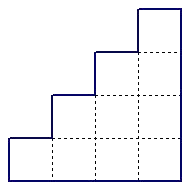
\includegraphics[scale=0.4]{06OMM4.png}
    \end{center}
\end{problem}
\begin{problem}
    [2008/4]
    Un rey decide realizar un juego para premiar a uno de sus caballeros, para ello, acomoda
a los $n$ caballeros en una mesa redonda y hace que digan los números $1, 2, 3$ y repitan de
nuevo $1, 2, 3$ y así sucesivamente (lo dicen en el sentido de las manecillas del reloj y cada
persona dice un número). Las personas que dicen $2$ ó $3$ son retiradas inmediatamente y
el juego continúa hasta que queda un sólo caballero, el ganador. Se numeran las personas
del $1$ al $n$ conforme al primer turno.
Encuentra todos los valores de $n$ de tal manera que el ganador sea el caballero $2008$.
\end{problem}
\begin{problem}
    [2010/4] Sea $n$ un entero positivo. En una cuadricula de $n\times 4$, cada region es igual a 
    $$\fbox{2}\fbox{0}\fbox{1}\fbox{0}$$
    Un "cambio" es tomar tres casillas consecutivas en el mismo renglón y con dígitos distintos escritos en ellas y cambiar los tres dígitos de estas casillas escritas de la siguiente manera.
    $$0\rightarrow 1 \text{, }1\rightarrow 2 \text{, }2\rightarrow 0$$
    Por ejemplo, un renglon $\fbox{2}\fbox{0}\fbox{1}\fbox{0}$ puede cambiarse al renglon $\fbox{0}\fbox{1}\fbox{2}\fbox{0}$ pero no al renglon $\fbox{2}\fbox{1}\fbox{2}\fbox{1}$ pues 0,1y 0 no son distintos entre sí. Los cambios se pueden aplicar cuantas veces se quiera, aún a renglones ya cambiados. Muestra que para $n<12$ no es posible hacer un número finito de cambios de forma que la suma de los numeros en cada una de las cuatro columnas sea la misma. 
\end{problem}
\begin{problem}
    [2011/1] 
    Se tienen 25 focos distribuidos de la siguiente manera: los primeros 24 se disponen en una
circunferencia colocando un foco en cada uno de los vértices de un 24-ágono regular, y el
foco restante se coloca en el centro de dicha circunferencia.
Se permite aplicar cualquiera de las siguientes dos operaciones:

1) Tomar dos vértices sobre la circunferencia tales que hay una cantidad impar de
vértices en los arcos que definen, y cambiar el estado de los focos de estos dos
vértices, así como del foco del centro.

2)Tomar tres vértices sobre la circunferencia que formen un triángulo equilátero, y
cambiar el estado de los focos en estos tres vértices, así como del foco del centro.

Muestra que partiendo de cualquier configuración inicial de focos encendidos y apagados,
siempre es posible llegar a una configuración en la que todos los focos están encendidos.
\end{problem}
\begin{problem}
    [2013/4] 
    Un cubo de $n \times n \times n$ está construido con cubitos de $1 \times 1 \times 1$, algunos negros y otros blancos, de manera que en cada uno de los subprismas de $n\times 1\times 1$, de $1\times n\times 1$ y de $1\times 1\times n$ hay exactamente dos cubitos negros y entre ellos hay un número par (posiblemente $0$) de cubitos blancos intermedios. Por ejemplo, en la ilustración, se muestra una posible rebanada del cubo de $6 \times 6 \times 6$ (formada por $6$ subprismas de $1 \times 6 \times 1$). Muestra que es posible sustituir la mitad de los cubitos negros por cubitos blancos para que en cada subprisma de $n \times 1 \times 1$, de $1 \times n \times 1$ y de $1 \times 1 \times n$ haya exactamente un cubito negro. \\
    \begin{center}
    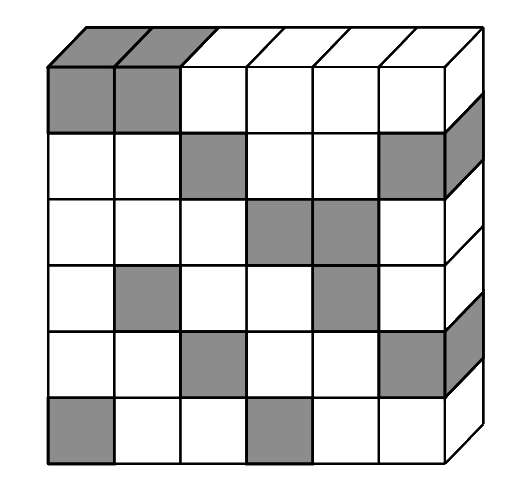
\includegraphics[scale=0.2]{13OMM4.png}
    \end{center}
\end{problem}
\begin{problem}
    [2014/1]  Cada uno de los números del $1$ al $4027$ se ha coloreado de verde o de rojo. Cambiar el color de un número es pasarlo a verde si era rojo, y pasarlo a rojo si era verde. Diremos que dos enteros positivos $m$ y $n$ son "cuates" si alguno de los números $\frac m n$ o $\frac n m$ es un número primo. Un paso consiste en elegir dos números que sean cuates y cambiar el color de cada uno de los números. Muestra que después de realizar algunos pasos es posible hacer que todos los números del $1$ al $2014$ sean verdes.
\end{problem}
\begin{problem} [2017/1]
    
    En un tablero de ajedrez de $2017 \times 2017$, se han colocado en la primera columna $2017$
caballos de ajedrez, uno en cada casilla de la columna. Una tirada consiste en elegir dos
caballos distintos y de manera simulátnea moverlos como se mueven los caballos de ajedrez.
Encuentra todos los posibles valores enteros de $k$ con $1 \leq k \leq 2017$, para los cuales es
posible llegar a través de varias tiradas, a que todos los caballos están en la columna $k$, uno
en cada casilla.
Nota. Un caballo se mueve de una casilla $X$ a otra $Y$, solamente si $X$ y $Y$ son las esquinas
opuestas de un rectángulo de $3 \times 2$ o de $2 \times 3$.
\end{problem}
\begin{problem}
    [2020/4] 
    Sea $n\ge 3$ un número entero. En un juego hay $n$ cajas en un círculo. Al principio, cada caja contiene un objeto que puede ser piedra, papel o tijeras, de forma que no hay dos cajas adyacentes con el mismo objeto, y cada objeto aparece en al menos una caja. 

Al igual que en el juego, piedra gana a tijera, tijera gana a papel y papel gana a piedra.   

El juego consiste en mover objetos de una caja a otra según la siguiente regla:  

Se eligen dos cajas adyacentes y un objeto de cada una de ellas de forma que sean diferentes, y movemos el objeto perdedor a la caja que contiene el objeto ganador. Por ejemplo, si elegimos una piedra de la caja A y unas tijeras de la caja B, movemos las tijeras a la caja A. 

Demuestra que, aplicando la regla suficientes veces, es posible mover todos los objetos a la misma caja.
\end{problem}
\begin{problem}
    [2022/4] 
    Sea $n$ un entero positivo. En un jardín de $n\times n$ cuyos lados dan al Norte, Sur, Este y Oeste, se va a construir una fuente usando plataformas de $1\times 1$ que cubran todo el jardín. Ana colocará las plataformas todas a diferentes alturas. Después, Beto pondrá salidas de agua en algunas de las plataformas. El agua de cada plataforma puede bajar a las plataformas contiguas (hacia el Norte, Sur, Este y Oeste) que tengan menor altura que la plataforma de donde viene el agua, siguiendo su flujo siempre que pueda dirigirse a plataformas de menor altura. El objetivo de Beto es que el agua llegue a todas las plataformas. ¿Cuál es el menor número de salidas de agua que Beto necesita tener disponibles a fin de garantizar que podrá lograr su objetivo, sin importar cómo Ana haya acomodado las plataformas?
\end{problem}
\begin{problem}[2023/4]
    Dada una coleccion de $n$ fichas que pueden estar pintadas de negro o blanco, tienen cada ficha un numero del $1$ al $n$ escrito. Un mago puede hacer los siguientes movimientos: elige $2$ fichas y convierte la ficha con el menor numero en una copia de la mayor (mismo color y numero).
El mago va a jugar haciendo estos movimientos hasta que ya no pueda hacer mas movimientos. 
Si consideras todas las maneras en que puede jugar y con los colores en que puede empezar, cuales son los posibles numeros de movimientos que puede hacer el mago?
\end{problem}
\subsection{P2-5}
\begin{problem}
    [2000/2]
    Se construye un triángulo de números de la siguiente manera. La primera fila está formada por los números de $1$ a $2000$ en orden creciente, y debajo de dos números consecutivos cualesquiera se escribe su suma. ¿Cuál es el número de la última fila? 
\end{problem}
\begin{problem}
    [2000/5]
    Un tablero $n$×$n$ está coloreado en blanco y negro como un tablero de ajedrez. Se pueden realizar los siguientes pasos: Elegir un rectángulo dentro del tablero (formado por casillas enteras) cuyas longitudes de los lados sean ambas impares o ambas pares, pero no ambas iguales a $1$, e invertir los colores de todas las casillas dentro del rectángulo. Determinar los valores de $n$ para los que es posible hacer que todas las celdas tengan el mismo color en un número finito de dichos pasos. 
\end{problem}
\begin{problem}
    [2001/2]
    Se tienen algunas pelotas de colores (son por lo menos tres colores), y por lo menos tres cajas. Las pelotas se ponen en las cajas de manera que no quede vacía ninguna caja y que no haya tres pelotas de colores distintos que estén en tres cajas distintas. Muestra que hay una caja tal que todas las pelotas que están fuera de ella son del mismo color.
\end{problem}
\begin{problem}
    [2003/5]
    Se escriben en tarjetas todas las parejas de números enteros $(a,b)$ con $1\leq a < b\leq 2003$. Dos personas juegan con las tarjetas como sigue; cada jugador en su turno elige $(a,b)$ (que se retira del juego) y escribe el producto $a\cdot b$ en un pizarrón (ambos jugadores usan el mismo pizarrón). Pierde el jugador que ocasione que el máximo común divisor de los números escritos hasta el momento sea $1$. ¿Quién tiene estrategia ganadora? (Es decir, ¿cuál de los dos jugadores puede inventar un método con el cual asegura su triunfo?). 
\end{problem}
\begin{problem}
    [2005/2]
    Dadas varias cuadrículas del mismo tamaño con números escritos en sus casillas, su suma se efectúa sumando las casillas que están en la misma posición, creando una cuadrícula del mismo tamaño.
Dado un entero positivo $N$, diremos que una cuadrícula es $N$-balanceada si tiene números enteros escritos en sus casillas y si la diferencia entre los números escritos en cualesquiera dos casillas que comparten un lado es menor o igual a $N$. Muestra que toda cuadrícula $2n$-balanceada (de cualquier tamaño) se puede escribir como suma de dos cuadrículas $n$-balanceadas. A demás, muestra que toda cuadrícula $3n$-balanceada (de cualquier tamaño) se puede escribir como suma de tres cuadrículas $n$-balanceadas.
\end{problem}
\begin{problem}
    [2007/5] 
    En cada cuadrado de una cuadrícula de $6 \times 6$ hay una luciérnaga apagada o encendida.
Una movida es escoger tres cuadrados consecutivos ya sean los tres verticales o los tres
horizontales, y cambiar de estado a las tres luciérnagas que se encuentran en dichos
cuadrados. Cambiar de estado a una luciérnaga significa que si está apagada se enciende
y viceversa.
Muestra que si inicialmente hay una luciérnaga encendida y las demás apagadas, no es
posible hacer una serie de movidas tales que al final todas las luciérnagas estén apagadas.
\end{problem}
\begin{problem}
    [2010/2]
    En cada casilla de un tablero de $n \times n$ hay un foco. Inicialmente todos los focos están
apagados. En un paso, se permite cambiar el estado de todos los focos en una fila o de
todos los focos en una columna (los focos prendidos se apagan y los focos apagados se
prenden).
Muestra que si después de cierta cantidad de pasos hay uno o más focos prendidos entonces
en ese momento hay al menos $n$ focos prendidos.
\end{problem}
\begin{problem}
    [2011/5] 
    Considera un tablero de $(2^n - 1) \times (2^n + 1)$ casillas que se quiere dividir en rectángulos
de tal forma que los lados de los rectángulos sean paralelos a los lados del tablero, de
tal forma que el área (cantidad de casillas) de cada rectángulo sea una potencia de $2$.
Encuentra la menor cantidad de rectángulos en las que se puede dividir el tablero.
\end{problem}
\begin{problem}
    [2012/2]
    Sea $n \geq 4$ un número par. Considera una cuadrícula de $n \times n$. Dos celdas (cuadritos
de $1 \times 1$) son vecinas si comparten un lado, si están en extremos opuestos de un mismo
renglón o si están en extremos opuestos de una misma columna. De esta forma, toda celda
en la cuadrícula tiene exactamente cuatro celdas vecinas.
En cada celda está escrito un número del $1$ al $4$ de acuerdo con las siguientes reglas:

Si en una celda está escrito un $2$ entonces en dos o más celdas vecinas está escrito
un $1$.

Si en una celda está escrito un $3$ entonces en tres o más celdas vecinas está escrito
un $1$.

Si en una celda está escrito un $4$ entonces en las cuatro celdas vecinas está escrito
un $1$.

Entre los acomodos que cumplan las condiciones anteriores, ¿cual el máximo número que
se puede obtener sumando los números escritos en todas las celdas?
\end{problem}
\begin{problem}
    [2012/5]
    Algunas ranas, unas de ellas rojas y otras verdes, se van a mover en un tablero de $11 \times 11$,
de acuerdo a las siguientes reglas. Si una rana está ubicada, digamos, en la casilla marcada
con $\#$ en la siguiente figura, entonces si es roja, puede saltar a cualquiera de las casillas marcadas con $\times$. Si es verde, puede saltar a cualquiera de las casillas marcadas con $\circ$.
Diremos que dos ranas (de cualquier color) se pueden encontrar en una casilla si ambas
pueden llegar hasta ella saltando una o más veces, no necesariamente con el mismo número
de saltos.
(a) Muestra que si ponemos $6$ ranas (de cualquier color), entonces hay al menos $2$ que se
pueden encontrar.
(b) ¿Para qué valores de $k$ es posible poner una rana roja y una rana verde de manera
que haya exactamente $k$ casillas en las que estas ranas se pueden encontrar?
    \begin{center}
        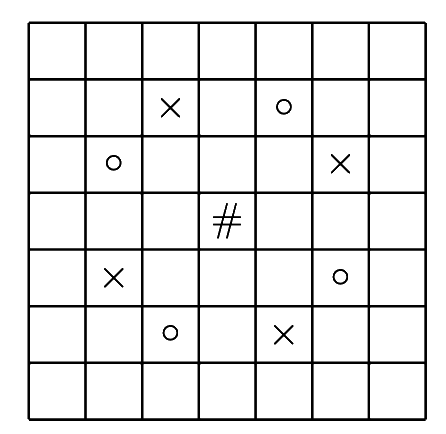
\includegraphics[scale=0.3]{12OMM5.png}
    \end{center}
\end{problem}
\begin{problem}
    [2015/2]
    Sea $n$ un entero positivo y $k$ un entero entre $1$ y $n$. Se tiene un tablero de $n \times n$ color blanco. Se hace el siguiente proceso. Se dibujan $k$ rectángulos con lados de longitud entera, con lados paralelos a los del tablero y tales que su esquina superior derecha coincide con la del tablero. Luego, estos $k$ rectángulos se rellenan de negro. Esto deja una figura blanca en el tablero.
¿Cuántas figuras blancas diferentes podemos obtener, que no se puedan obtener haciendo el proceso con menos de $k$ rectángulos?

Nota: A continuación se muestra un ejemplo para un tablero de $6 \times 6$. Se dibujan $3$ rectángulos, uno de $1 \times 5$, uno de $2 \times 4$ y uno de $4 \times 2$, para obtener la figura blanca indicada en el tablero de la derecha.
    \begin{center}
        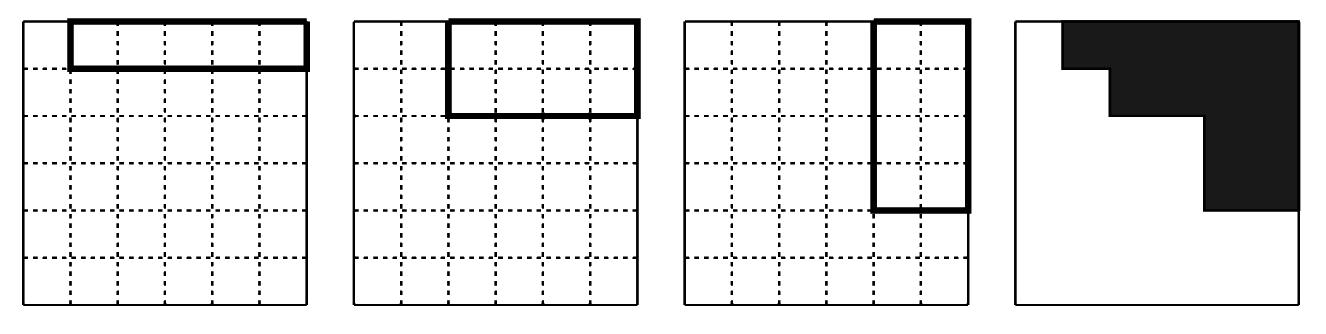
\includegraphics[scale=0.3]{15OMM2.png}
    \end{center}
\end{problem}
\begin{problem}
    [2016/5]
    En una cuadrícula de $n \times n$ se escriben los números del $1$ al $n^2$ en orden, por renglones,
de manera que en el primer renglón aparecen los números del $1$ al $n$, en el segundo los
números de $n + 1$ a $2n$, y así sucesivamente. Una operación permitida en la cuadrícula
consiste en escoger cualesquiera dos cuadraditos que compartan un lado y sumar (o restar)
el mismo número entero a los dos números que aparecen en esos cuadraditos. Por ejemplo, abajo se muestran dos operaciones sucesivas permitidas en una cuadrícula de $4 \times 4$:
primero restando $7$ a los cuadraditos sombreados y luego sumando $5$ a los sombreados.

Determina para qué valores de $n$ es posible lograr que todos los cuadraditos tengan escrito
el número $0$ después de repetir la operación tantas veces como sea necesario y, en los casos
en que sea posible, determina el mínimo número de operaciones necesarias.
    \begin{center}
        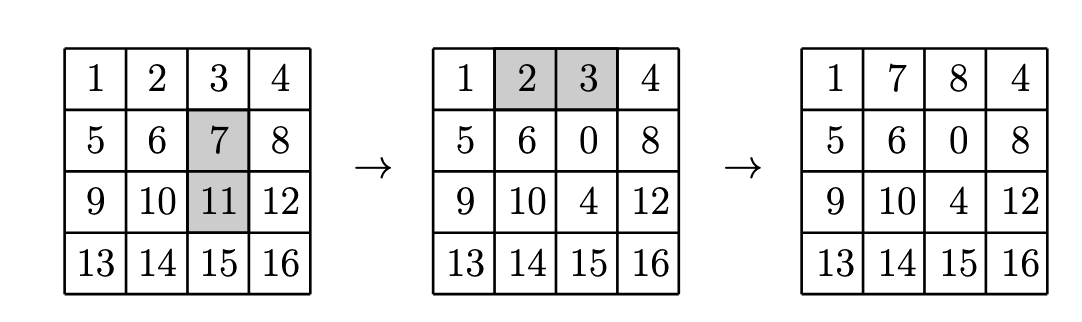
\includegraphics[scale=0.3]{16OMM5.png}
    \end{center}
\end{problem}
\begin{problem}
    [2018/2]
    Para cada número entero positivo $m$, definimos $L_m$ como la figura que se obtiene al superponer dos rectángulos de $1 \times 1$ y $m\times 1$ de manera que coincidan en el cuadrado de $1 \times 1$ en sus extremos, como se muestra en la figura.

Utilizando unas figuras $L_{m_1}, L_{m_2}, \dots, L_{m_k}$, cubrimos completamente un tablero $n \times n$, de forma que las aristas de la figura coincidan con líneas del tablero. Entre todas las coberturas posibles del tablero, encontrar el mínimo valor posible de $m_1 + m_2 + \dots + m_k$.

Nota: Al cubrir el tablero, las figuras pueden estar giradas o reflejadas, y pueden solaparse o no estar completamente contenidas en el tablero.
    \begin{center}
        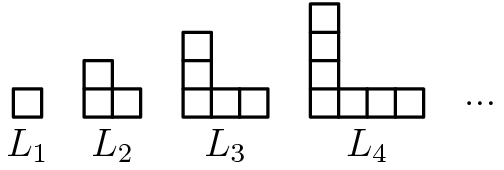
\includegraphics[scale=0.3]{18OMM2.png}
    \end{center}
\end{problem}
\begin{problem}
    [2019/5]
    Sean $a > b$ enteros positivos relativamente primos. Un saltamontes se sitúa en el punto $0$ de una recta numérica. Cada minuto, el saltamontes salta de acuerdo con las siguientes reglas:

    Si el minuto actual es un múltiplo de $a$ y no un múltiplo de $b$, salta $a$ unidades hacia adelante.
    Si el minuto actual es un múltiplo de $b$ y no un múltiplo de $a$, salta $b$ unidades hacia atrás.
    Si el minuto actual es tanto un múltiplo de $b$ como un múltiplo de $a$, salta $a - b$ unidades hacia adelante.
    Si el minuto actual no es ni un múltiplo de $a$ ni un múltiplo de $b$, no se mueve.

Encuentra todas las posiciones de la recta numérica que el saltamontes acabará alcanzando.

\end{problem}
\begin{problem}
    [2022/2] 
    Sea $n$ un entero positivo. David tiene $6$ tableros de ajedrez de $n\times n$ que ha dispuesto de manera que formen las $6$ cara de un cubo de $n\times n\times n$. Se dice que dos casillas $a$ y $b$ están alineadas si están en una misma fila o columna en un tablero o continuan así por los tableros adyacentes. David coloca algunas torres en el tablero de forma que no se ataquen entre sí. Dos torres se atacan entre sí si están en casillas alineadas. ¿Cuál es la máxima cantidad de torres que David puede colocar?
\end{problem}
\begin{problem} [2023/2]
    Los números del 1 al 2000 se encuentran colocados sobre los vertices de un poligono regular de 2000 lados, uno en cada vertice, de manera que se cumple lo siguiente: 
    Si cuatro enteros $1 \leq A < B < C < D \leq 2000$ entonces el segmento que une los vertices donde estan los numeros $A$ y $B$, y el segmento que une los vertices donde estan los numeros $C$ y $D$ no se intersecan en el interior del poligono.  \\
    Demuestra que existe un entero positivo que es un numero cuadrado perfecto tal que el numero diametralmente opuesto a el no es un cuadrado perfecto.
\end{problem}
\subsection{P3-6} 
\begin{problem}
    [2001/6] 
    Un coleccionista de monedas raras tiene monedas de denominaciones $1,2,3,\dots,n$ (tiene muchas monedas de cada denominación). Desea poner algunas de sus monedas en $5$ cajas de manera que se cumplan las siguientes condiciones:

a) En cada caja hay a lo más una moneda de cada denominación.

b) Todas las cajas tienen el mismo número de monedas y la misma cantidad de dinero.

c) Para cualesquiera dos cajas sucede que entre las dos tienen por lo menos una moneda de cada denominación.

d) No existe una denominación tal que todas las cajas tengan una moneda de esta denominación

¿Para qué valores de $n$ puede el coleccionista hacer lo que se propone?
\end{problem}
\begin{problem}
    [2003/3]
    En una fiesta hay el mismo número $n$ de muchachos que de muchachas. Supón que a cada muchacha le gustan $a$ muchachos y a cada muchacho le gustan $b$ muchachas. Para qué valores de $a$ y $b$ es correcto afirmar que hay un muchacho y una muchacha que se gustan mutuamente?
    
\end{problem}
\begin{problem}
    [2004/6] 
    ¿Cuál es el mayor número posible de cambios de dirección en un recorrido sobre las líneas de una cuadrícula de $2004\times 2004$ casillas, si el recorrido no pasa dos veces por el mismo lugar?
\end{problem}
\begin{problem}
    [2006/3]
    Sea $n$ un número entero mayor que $1$. ¿De cuántas formas se pueden acomodar todos los números $1,2,3,\dots 2n$ en las casillas de una cuadrícula de $2\times n$, uno en cada casilla, de manera que cualesquiera dos números consecutivos se encuentren en casillas que comparten un lado en la cuadrícula?
\end{problem}
\begin{problem}
    [2008/3]
    Considera un tablero de ajedrez. Los números del $1$ al $64$ se escriben en las casillas del
tablero como en la figura. Se disponen de suficientes caballos de ajedrez para colocarlos en las casillas del tablero de
manera que no se ataquen entre sí. Calcula la suma de los números de las casillas donde
están colocados los caballos. ¿Cuál es la suma máxima que puedes obtener? Nota. Dos
caballos se atacan entre sí, cuando se encuentran en 2 esquinas opuestas de un rectángulo
de $2\times 3$ o de $3 \times 2$.
\end{problem}
\begin{problem}
    [2009/6]
    En una fiesta con $n$ personas, se sabe que de entre cualesquiera $4$ personas, hay $3$ de las
$4$ que se conocen entre sí o hay $3$ que no se conocen entre sí. Muestra que las $n$ personas
se pueden separar en dos salones de manera que en un salón todos se conocen entre sí y
en el otro no hay dos personas que se conozcan entre sí.
Nota. Conocerse se considera una relación mutua.
\end{problem}
\begin{problem}
    [2017/6] 
    Sean $n \geq 2$ y $m \geq 2$ enteros positivos. Se tienen $m$ urnas dispuestas en fila. Los jugadores
$A$ y $B$ juegan por turnos, comenzando por $A$, de la siguiente manera. En cada turno, $A$
elige dos urnas y coloca un voto en cada una de ellas. Posteriormente, $B$ elige una urna,
y elimina todos los votos de esa. $A$ gana si logra que haya una urna con $n$ votos después
de algún turno de $B$. Determina para cada $n$ el mínimo valor de $m$ para el cual $A$ puede
garantizar ganar, sin importar los movimientos que haga $B$.
\end{problem}
\begin{problem}
    [2019/3] 
    Sea $n\geq 2$ un número entero. Considera $2n$ puntos alrededor de un círculo. Cada vértice se ha marcado con un número entero desde $1$ hasta $n$, inclusive, y cada uno de estos enteros se ha utilizado exactamente dos veces. Isabel divide los puntos en $n$ pares, y dibuja los segmentos que los unen, con la condición de que estos segmentos no se crucen. A continuación, asigna a cada segmento el mayor número entero entre sus puntos extremos. Muestra que, independientemente de cómo se hayan marcado los puntos, Isabel siempre puede elegir los pares de forma que utilice exactamente $\lceil n/2\rceil$ números para marcar los segmentos. ¿Se pueden etiquetar los puntos de tal manera que, independientemente de cómo Isabel divida los puntos en pares, siempre utilice exactamente $\lceil n/2\rceil$ números para etiquetar los segmentos?

Nota: Para cada número real $x$, $\lceil x\rceil$ denota el menor número entero mayor o igual que $x$. Por ejemplo, $\lceil 3,6\rceil=4$ y $\lceil 2\rceil=2$.
\end{problem}
\begin{problem}
    [2020/3] 
    Sea $n\ge 3$ un número entero. Dos jugadores, Ana y Beto, juegan al siguiente juego. Ana etiqueta los vértices de un $n$-ágono regular con los números del $1$ al $n$, en el orden que quiera. Cada vértice debe ser etiquetado con un número diferente. A continuación, colocamos un guajolote en cada uno de los $n$ vértices.  \newline 
Estos guajolotes se entrenan para lo siguiente. Si Beto silba, cada guajolote se mueve al vértice adyacente con mayor etiqueta. Si Beto aplaude, cada guajolote se mueve al vértice adyacente con la etiqueta menor.  \newline 
Beto gana si, tras un cierto número de silbidos y palmadas, consigue mover todos los guajolotes al mismo vértice. Ana gana si consigue etiquetar los vértices para que Beto no pueda hacerlo. Para cada $n\ge 3$, determina qué jugador tiene una estrategia ganadora.
\end{problem}
\begin{problem}
    [2021/3] 
    Sean $m,n\geq 2$ dos enteros. En una cuadrícula de $m\times n$, una hormiga empieza en el cuadrito inferior izquierdo y quiere caminar al camino superior derecho. Cada paso que da la hormiga debe ser a un cuadrito adyacente, y de acuerdo a las siguientes posibilidades: $\uparrow$, $\rightarrow$ y $\nearrow$. Sin embargo, un malvado mago ha dejado caer lava desde arriba de la cuadrícula y ha destruido algunos cuadritos, de forma tal que:
 \begin{itemize} 
 \item Si un cuadrito está destruido, entonces todos los cuadritos superiores a él también también están destruidos.

 \item El número de cuadritos destruidos es mayor o igual a $0$.

 \item Quedan suficientes cuadritos sin destruir para que la hormiga pueda llegar a la meta. 
 \end{itemize} 
Sea $P$ el número de caminos de longitud par que puede seguir la hormiga. Sea $I$ el número de caminos de longitud impar que puede seguir la hormiga. Encuentra todos los posibles valores de $P-I$.
    \begin{center}
        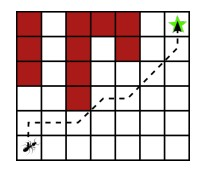
\includegraphics[scale=0.6]{21OMM3.jpg}
    \end{center}
\end{problem}
\begin{problem}
    [2021/6] 
    Determina todos los conjuntos no vacíos $C_1, C_2, C_3, \cdots $ tales que cada uno de ellos tiene un número finito de elementos, y todos sus elementos son enteros positivos, con la siguiente propiedad: Para cualesquiera enteros positivos $n$ y $m$, el número de elementos del conjunto $C_n$ más el número de elementos del conjunto $C_m$ es igual a la suma de los elementos del conjunto $C_{m + n}$.
\end{problem}
\end{document}
